\section{Database og Data Access Layer}\label{sec:designdatabase}

%\subsection{Indledende design overvejelser}
Før design af database og data access layer, er der foretaget nogle indledende teknologiundersøgelser.

\subsection{Indledende overvejelser}
Lige fra starten har det været klart at systemet skulle udvikles i flere faser, jf. den agile tankegang. Databasen og data access laget er derfor udviklet sideløbende med resten af systemets funktionalitet.

Projektets mange iterationer kan deles op i tre faser, hvor det i første fase var målet at kunne oprette en bruger/User, og samtidig lave forespørgsler på databasen.
DDS-Lite\todo{Lav en reference til udviklingsværktøjer} blev brugt i første forsøg med at oprette en funktionel database til at gemme brugere og brugerinformation. Dette viste sig og at være en uholdbar løsning da systemet løbende skulle opdateres. I forbindelse med kurset I4DAB, blev der lavet en opgave hvor Entity Frameworket blev brugt. Dette framework gør det let at udvide systemet, hvilket passer godt til den iterative tilgang der er brugt i projektet. Entity Frameworket er en \textit{Object Relational Mapper}, der gør det lettere at arbejde med rå datarecords i et objekt orienteret system. Entity Frameworket gør det med andre ord muligt at behandle rå data records som objekter.

I grove træk vises Entity Frameworkets overordnede virkemåde på figur~\ref{fig:EFarch}, det skal nævnes at ''Application'' på figuren symbolisere data-access laget.

\begin{figure}[H]
\centering
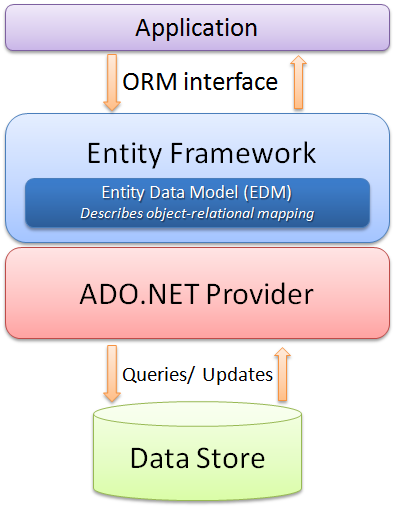
\includegraphics[width=0.5\linewidth]{figs/dbExtra/EFarch}
\caption{Entity Framework \cite{efArch}, hvor ''Application'' på diagrammet er DAL i systemet.}
\label{fig:EFarch}
\end{figure}


Helt fra begyndelsen af databasen og data-access lagets designfase, har tanken været at skabe en software komponent, der blot eksponerer et interface, der skal gøre det nemt for klienter at bruge det. Der er lavet et dependancy diagram som kan ses på figur~\ref{fig:vs_codeMap}.

Efter Entity Framkeworket blev vedtaget til brug, blev der udarbejdet et \textit{entity relationship} diagram ved hjælp af Visual Studio's modelling project. Der er flere måder at designe databaser på med Entity Frameworket og Visual Studio, hvor flere af dem blevet afprøvet undervejs, herunder \textit{Code First}, \textit{Model First} samt \textit{Database First}.

\textit{Database first} blev brugt i forlængelse med DDS-Lite, som blev brugt til at designe selve databasen og SQL scriptet til at lave tabellerne. Code First tilgangen gav en bred forståelse for hvordan Entity Frameworket fungerede, netop fordi at der ikke autogenereres klasser til entiteterne. Se figur~\ref{fig:generatedFiles} hvor entitetsklasser vises.

Dog blev \textit{Model First} tilgangen valgt, da der i projektets udviklingsfase ofte blev foretaget markante ændringer i designet. \textit{Model first} gør det lettere at udføre ER opdateringer, direkte på modellen og derefter køre et tilhørende SQL script direkte på databasen. 

Når der skal oprettes en database model, tilføjes der en \textit{ADO.NET Entity Data Model}. Model designeren bruges da til at tilføje, fjerne og ændre i entities.
På figur~\ref{fig:modelDesigner} vises brugen af designeren i projektet.

\begin{figure}
	\centering
	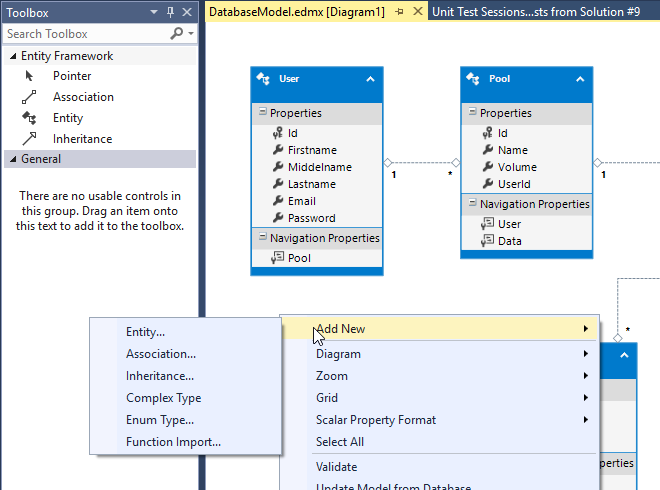
\includegraphics[width=\linewidth]{figs/modelDesigner}
	\caption{Eksempel på entity klasserne i projektet}
	\label{fig:modelDesigner}
\end{figure}

\begin{figure}
\centering
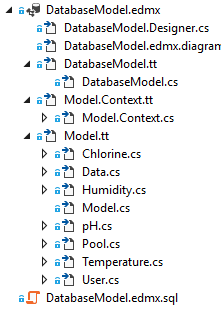
\includegraphics[width=0.35\linewidth]{figs/generatedFiles}
\caption{Eksempel på entity klasserne i projektet}
\label{fig:generatedFiles}
\end{figure}

Når der udvikles en database med \textit{Model First} tilgangen, autogenereres de simple entity klasser (User, Pool Data osv.). Dette er klart at foretrække når systemet er under udvikling idet model designeren selv kan opdatere klasserne når databasemodellen opdateres eller udvides. På denne måde undgås det at man selv skal ind og ændre alle entity klasserne manuelt. På figur~\ref{fig:generatedFiles} ses et eksempel på nogen af de autogenerede klasser.

Det første \textit{Model first} udkast til projektets database var meget omfattende og blev lavet før de første rigtige iterationer begyndte. Grunden til at denne databasemodel blev lavet var at tankegangen med at definere hele systemet fra starten af ikke var "sluppet" helt. Modellen er sidenhen blevet revideret og omkonstrueret. Se figur~\ref{fig:databaseERD_firstattempt_uml} for dette tidlige design.

\begin{figure}[h]
	\centering
	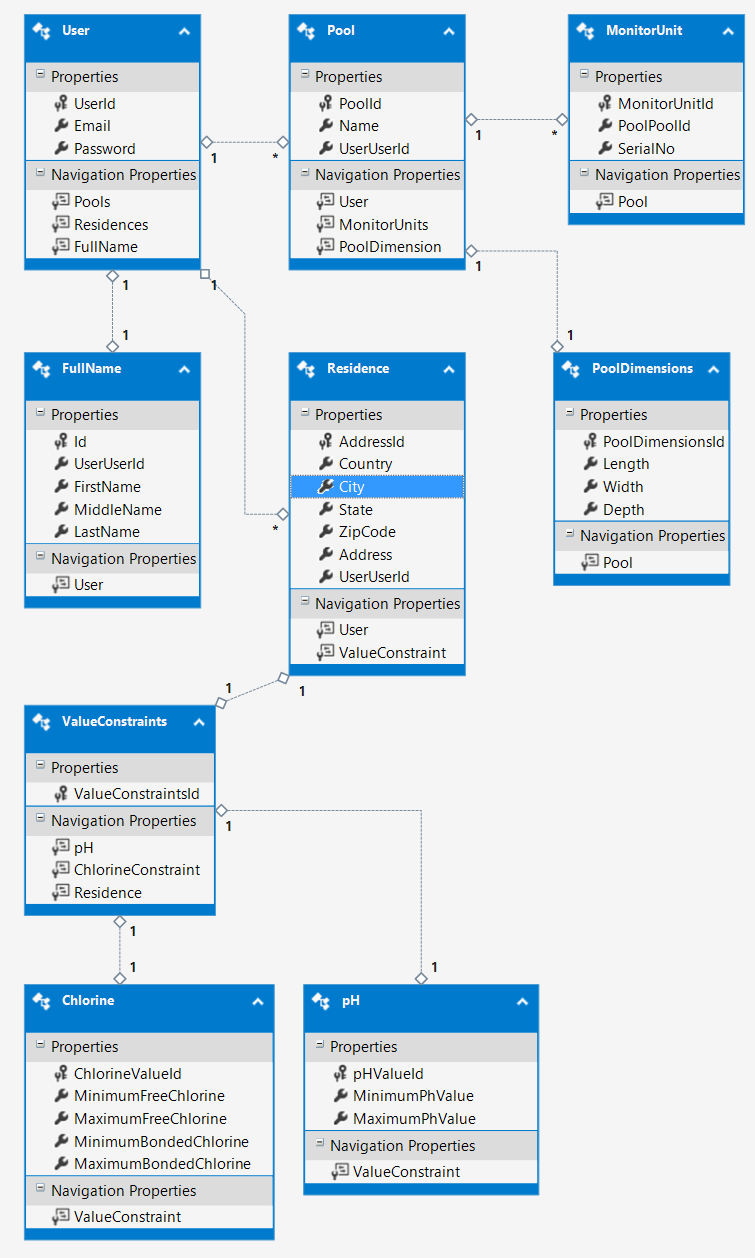
\includegraphics[width=0.8\linewidth]{figs/design/databaseERD}
	\caption{Første "Model First tilgang" til database design}
	\label{fig:databaseERD_firstattempt_uml}
\end{figure}

I løbet af udviklingsprocessen, dvs. fra projektets begyndelse til slutningen, er der foretaget mange ændringer af modellen der ses på figur~\ref{fig:databaseERD_firstattempt_uml}. 
I takt med at man tilegnede sig mere viden omkring database design blev der foretaget flere justeringer. Af markante ændringer kan der nævnes:

\begin{itemize}
	\item FullName entiteten fjernes, User får 3 naming properties.
	\item Residence entiteten fjernes, og Pool entitens \textit{Name} property står for indhold af både addresse og navn.
	\item Value constraints fjernes helt da de ikke er nødvendige at have på databasen
	\item PoolDimensions entiteten fjernes, og Pool får en \textit{Volume} property.
	\item MonitorUnit entiteten udgår af fra databasen. Denne har kun været i databasen for at checke på et evt. serienummer.
	\item Persistering af data er blevet smartere, se figur \ref{fig:databaseERD_final_uml}.
\end{itemize}

\begin{figure}[h]
	\centering
	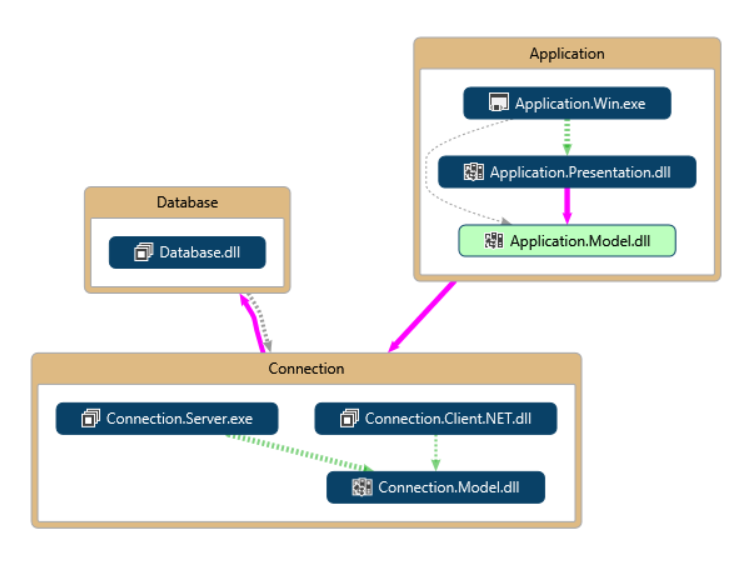
\includegraphics[width=0.8\linewidth]{figs/design/vs_codeMap.PNG}
	\caption{Dependancy graf for Smartpool Systemet}
	\label{fig:vs_codeMap}
\end{figure}

\begin{figure}
\centering
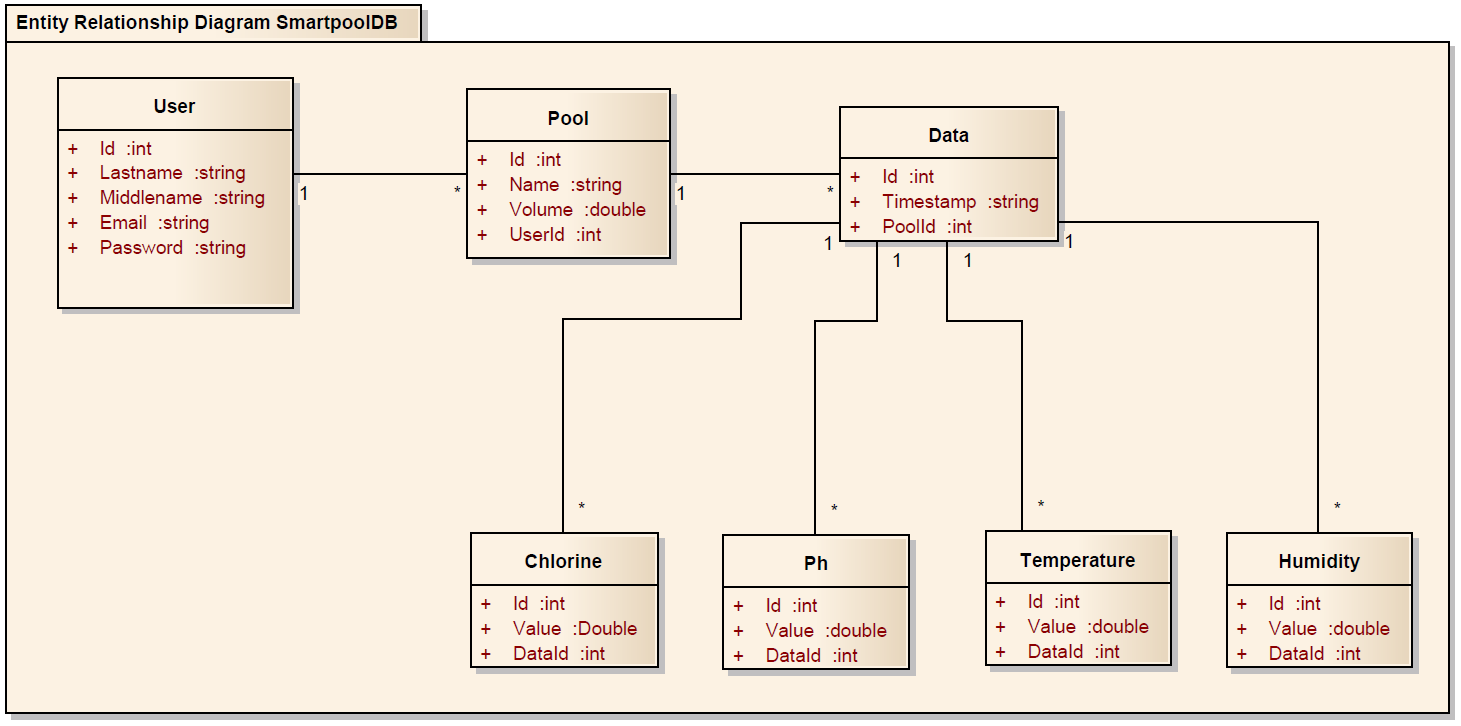
\includegraphics[width=0.7\linewidth]{figs/databaseERD_final_uml}
\caption{Entity Relationship Diagram for det endelige database design}
\label{fig:databaseERD_final_uml}
\end{figure}


\subsection{User Stories}
Herunder vil databasen og data-access lagets funktionalitet blive beskrevet ud fra de undervejs opstillede \textit{user stories}, herunder:

\begin{itemize}
	\item Som bruger vil jeg kunne oprette mig i systemet for at få adgang til systemet.
	\item Som administrator vil jeg kunne slette en bruger for at undgå spild af plads i databasen.
	\item Som bruger vil jeg kunne logge ind i systemet for at se mine data.
	\item Som bruger vil jeg kunne nulstille mit kodeord hvis jeg skulle glemme det.
	\item Som bruger vil jeg kunne ændre mit password for at sikre min konto.
	\item Som bruger vil jeg kunne tilføje en pool til min konto.
	\item Som bruger vil jeg kunne fjerne en pool fra min konto.
	\item Som bruger vil jeg kunne ændre informationer om en eksisterende pool på min konto.
	\item Som bruger vil jeg kunne se en liste over alle mine pools.
	\item Som bruger vil jeg kunne se de seneste sensor værdier for at kunne få et overblik over poolens tilstand.
\end{itemize}

\subsubsection{Oprettelse/ændring af brugere}
Herunder beskrives dokumentation for følgende \textit{user stories}:

\textit{"Som bruger vil jeg kunne oprette mig i systemet for at få adgang til systemet"}

\textit{"Som administrator vil jeg kunne slette en bruger for at undgå spild af plads i databasen"}

\textit{"Som bruger vil jeg kunne logge ind i systemet for at se mine data"}

Ud fra disse user stories, blev det besluttet af en bruger skulle have attributterne som vist på figur~\ref{fig:database_model_1}. Da entiteten er oprettet i databasen som en tabel, skulle data access laget nu designes så \gls{windserver} har adgang til brugerfunktionalitet.


\begin{figure}[H]
	\centering
	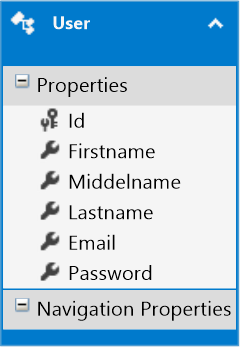
\includegraphics[width=0.25\linewidth]{figs/design/database_model_1}
	\caption{Model for første design for database-adgang.}
	\label{fig:database_model_1}
\end{figure}

Dette blev udviklet med \textit{Test Driven Development}, hvor der først blev skrevet enhedstest som testede følgende scenarier: 

\begin{lstlisting}[caption=Testcases til \textit{AddUser} metoden.,label=code:addusertestcases]
public void AddUser_InsertsUserWith3Names_UserHasCorrectFirstname()
public void AddUser_InsertsUserWith3Names_UserHasCorrectMiddelname()
public void AddUser_InsertsUserWith3Names_UserHasCorrectLastname()
public void AddUser_InsertUserWith2Names_UserHasCorrectFirstname()
public void AddUser_InsertUserWith2Names_UserHasCorrectLastname()
public void AddUser_AddingUserWith1NameOnly_ReturnsFalse()
public void AddUser_InsertUserWithAlreadyUsedEmail_ReturnsFalse()
public void AddUser_InsertUserWithAlreadyUsedEmail_SecondUserIsNotInDatabase()
public void AddUser_Add2UsersWithSameEmailWithDiffCaPiTaL_ReturnsFalse()
\end{lstlisting}

Et eksempel på implementeringen af en testcases, som sikre at der ikke kan sættes en bruger ind med et ''taget'' password, finders herunder. Øvrige testcases med implementering kan ses i vedlagt sourcekode i \textit{Smartpool} solutionen, \textit{Database.Test.Unit} projektet, i \textit{UserAccessUnitTest.cs} filen.

\begin{lstlisting}[caption=Test for metoden] AddUser_InsertUserWithAlreadyUsedEmail_ReturnsFalse]
...
[Test]
public void AddUser_InsertUserWithAlreadyUsedEmail_ReturnsFalse()
{
	_uut.AddUser("John Johnson", "mail", "password");
	
	Assert.That(_uut.AddUser("Derp Derpsen", "mail", "wordpass"), Is.False);
}
...
\end{lstlisting}

Disse blev udfærdiget og implementeret. Undervej blev der selvfølgelig fundet fejl i både test og kode, men tiden brugt på at rette fejlene på dette tidspunkt blev vurderet til at være væsentligt kortere end hvis de først blev fundet senere i processen. 

Endeligt kom \textit{AddUser} metoden til at se ud som vist på listing~\ref{code:adduser} og på grundet brugen af \textit{Test Driven Development} er det med en test-coverage på 100\%.

\begin{lstlisting}[caption=\textit{AddUser} metoden,label=code:adduser]
public bool AddUser(string fullname, string email, string password)
{
	if (IsEmailInUse(email)) return false;
	if (!ValidateName(fullname)) return false;
	
	User user;
	
	string[] names = fullname.Split(' ');
	
	if (names.Length <= 2)
	{
		user = new User() { Firstname = names[0], Lastname = names[1], Email = email, Password = password };
	}
	else
	{
		user = new User() { Firstname = names[0], Middelname = names[1], Lastname = names[2], Email = email, Password = password };
	}
	
	using (var db = new DatabaseContext())
	{
		db.UserSet.Add(user);
		db.SaveChanges();
	}
	
	return true;
}
\end{lstlisting}

Da metoden til at sætte en bruger ind i databasen var skrevet i data-access laget og samtidigt testet, skulle der implementeres funktionalitet til at hente denne bruger ud af databasen. Til dette blev følgende testcases designet:

\begin{lstlisting}[caption=Testcases til \textit{FindUserByEmail} metoden.,label=code:finduserbyemailtestcases]
public void FindUserByEmail_UserIsNotAdded_ReturnsNullUser()
public void FindUserByEmail_UserIsAdded_FindsCorrectUser()
public void FindUserByEmail_TwoUsersWithSameEmailInDB_ThrowsMultipleEmailsFoundException()
public void FindUserByEmail_InsertsUserWithEmailInAllCaps_FindUserSearchingWithLowerCaps()
\end{lstlisting}

Dette er lavet efter samme fremgangsmåde som beskrevet med \textit{AddUser} metoden. Sådan er funktionaliteten til at finde en bruger udviklet og på grund af dette igen med fuldstændigt testcoverage. Metoden er vist herunder: 

\begin{lstlisting}[caption=FindUserByEmail metode]
public User FindUserByEmail(string email)
{
	User foundUser;
	
	using (var db = new DatabaseContext())
	{
		var searchByEmail = from search in db.UserSet
				where search.Email.Equals(email)
				select search;
	
		if (searchByEmail.Count() > 1) 
			throw new MultipleOccourencesOfEmailWasFoundException();
		if (searchByEmail.Count() == 0) 
			throw new UserNotFoundException();
	
		foundUser = searchByEmail.First();
	}
	
	return foundUser;
}
\end{lstlisting}

Da \textit{FindUserByEmail} skal returnere en instans af \textit{User} klassen, var der begrænset mulighed for at gøre ''kalder'' klar over at en fejl var forekommet. Så \textit{FindUserByEmail} kaster en exception hvis kaldet mislykkedes.

Endeligt var der behov for at kunne verificere en brugers password. I forbindelse med dette var det vigtigt at selve kodeordet aldrig forlader data-access laget. Måden det blev implementeret på var at brugeren af metoden måtte sende email og kodeord med som argument, hvorefter \textit{ValidatePassword} skulle svare om disse matchede. Igen blev der fundet en række testcases:

\begin{lstlisting}[caption=Testcases til \textit{ValidatePassword} metoden.,label=code:validatepasswordtestcases]
public void ValidatePassword_ValidPassword_ReturnsTrue()
public void ValidatePassword_InvalidPassword_ReturnsFalse()
public void ValidatePassword_UserIsNotInDB_ReturnsFalse()
\end{lstlisting}

Disse blev skrevet og løbende blev \textit{ValidatePassword} implementeret, som vist herunder:

\begin{lstlisting}[caption=ValidatePassword metoden]
public bool ValidatePassword(string email, string password)
{
	User user;
	try
	{
		user = FindUserByEmail(email);
	}
	catch (Exception e)
	{
		Console.WriteLine("Herro pree, u can haz exception: " + e);
		return false;
	}
	
	if (user.Password == password) return true;
	
	return false;
}
\end{lstlisting}

\subsubsection{Nulstilling/ændring af password}
Herunder beskrives dokumentation for følgende \textit{user stories}:

\textit{"Som bruger vil jeg kunne nulstille mit kodeord hvis jeg skulle glemme det"}

\textit{"Som bruger vil jeg skulle ændre mit password for at sikre min konto"}

For at en bruger kan ændre sit password, skal der på User entiteten være en property til et kodeord, er allerede indsat på figur~\ref{fig:database_model_1}. Herefter er følgende testcases fundet: 

\begin{lstlisting}[caption=Testcases til EditUserPassword metoden]
public void EditUserPassword_ChangePasswordOfNotExistingUser_ReturnsFalse()
public void EditUserPassword_ChangeToInvalid_ReturnsFalse()
public void EditUserPassword_ChangePassword_ReturnsTrue()
\end{lstlisting}

Prioriteten ved denne metode var at det ikke skulle være muligt at fjerne sit kodeord, eller sætte det til en tom string. Implementering ses herunder.

\begin{lstlisting}[caption=EditUserPassword metoden]
public bool EditUserPassword(string email, string newPassword)
{
	if (!IsEmailInUse(email) || newPassword.Length == 0)
	{
		return false;
	}
	
	using (var db = new DatabaseContext())
	{
		var original = db.UserSet.Find(FindUserByEmail(email).Id);
		if (original != null)
		{
			original.Password = newPassword;
			db.SaveChanges();
		}
	}
	
	return true;
}
\end{lstlisting}

\subsubsection{Tilføjeselse/ændring af pools til bruger}

\textit{''Som bruger vil jeg kunne tilføje en pool til min konto''}

\textit{''Som bruger vil jeg kunne fjerne en pool fra min konto.''}

\textit{''Som bruger vil jeg kunne ændre informationer om en eksisterende pool på min konto.''}

\textit{''Som bruger vil jeg kunne se en liste over alle mine pools.''}

Omkring tilføjelse af pools var det vigtigt at en bruger ikke kan tildeles flere pools med det samme navn. Følgende test blev opstillet:

\begin{lstlisting}[caption=Testcases til AddPool metoden]
public void AddPool_AddingPoolWithInvalidName_ReturnsFalse()
public void AddPool_AddingPoolWithExistingUser_IsPoolNameAvailableReturnsFalse()
public void AddPool_AddingPoolWithValidUser_ReturnsNull()
public void AddPool_AddingPoolWithZeroVolume_ReturnsTrue()
public void AddPool_AddingPoolWithNeg5Volume_ReturnsFalse()
public void AddPool_AddingIdenticalPool_ReturnsFalse()
public void AddPool_AddingSecondPoolWithValidName_IsPoolNameAvailableReturnsTrue()
public void AddPool_AddingPoolToOtherUserWithSameName_ReturnTrue()
public void AddPool_AddingPoolToExistingUser_DoesNotThrowException()
public void AddPool_AddingPoolToExistingUser_UserOnlyAppearOnceInDb()
\end{lstlisting}

Samtidigt med at disse test med identificeret, blev selve implementering lavet. Implementeringen kan ses herunder: 

\begin{lstlisting}[caption=AddPool metoden]
public bool AddPool(string email, string name, double volume)
{
	if (name == "")	return false;
	if (IsPoolNameAvailable(email, name) == false)	return false;
	if (volume < 0)	return false;
	
	Pool newPool = new Pool { Name = name, Volume = volume, UserId = UserAccess.FindUserByEmail(email).Id };
	
	using (var db = new DatabaseContext())
	{
		db.PoolSet.Add(newPool);
		db.SaveChanges();
	}
	
	return true;
}
\end{lstlisting}

Til fjernelsen af en pool fra en bruger blev følgende testcases fundet:

\begin{lstlisting}[caption=Testcases til RemovePool metoden]
public void RemovePool_RemoveExistingPool_IsPoolNameAvailableReturnsTrue()
public void RemovePool_PoolNotInDatabase_RemovePoolReturnsFalse()
\end{lstlisting}

Samtidigt med at test blev fundet og skrevet blev selve implementering lavet og herunder ses det færdige resultat.

\begin{lstlisting}[caption=RemovePool metoden]
public bool RemovePool(string email, string name)
{
	if (IsPoolNameAvailable(email, name))return false;
	
	using (var db = new DatabaseContext())
	{
		var searchForPool = from pool in db.PoolSet
				where pool.Name == name
				select pool;
		
		foreach (Pool pool in searchForPool)
		{
			if (pool.UserId == UserAccess.FindUserByEmail(email).Id)
			{
				db.PoolSet.Remove(pool);
			}
		}
	
		db.SaveChanges();
	}
	
	return true;
}
\end{lstlisting}

\paragraph{Ændring af poolinformationer}

En pools attributter, kan alle ændre. I dette underafsnit vil ændringen af navnet for en pool blive gennemgået. For at lave funktionalitet til at ændre på poolinformationer blev følgende testcases først identificeret:

\begin{lstlisting}[caption=Testcases til EditPoolName metoden]
public void EditPoolName_ChangeNameOfNotExistingPool_ReturnsFalse()
public void EditPoolName_ChangeNameOfExistingPoolToInvalid_ReturnsFalse()
public void EditPoolName_ChangeNameOfExistingPoolToTakenName_ReturnsFalse()
public void EditPoolName_ChangeNameOfExistingPool_ReturnsTrue()
public void EditPoolName_ChangeNameOfExistingPoolTo_IsPoolNameAvailableReturnsTrue()                        
\end{lstlisting}

Samtidigt med at test blev fundet og skrevet blev selve implementering lavet og herunder ses det færdige resultat.

\begin{lstlisting}[caption=Metoden EditPoolName]
public bool EditPoolName(string ownerEmail, string currentName, string newName)
{
	if (newName == "") return false;
	if (!IsPoolNameAvailable(ownerEmail, newName)) return false;
	
	using (var db = new DatabaseContext())
	{
		var searchForPool = from pool in db.PoolSet
				where pool.User.Email == ownerEmail && pool.Name == currentName
				select pool;
		
		if (searchForPool.Any() == false) return false;
		
		searchForPool.First().Name = newName;
		
		db.SaveChanges();
	}
	
	return true;
}
\end{lstlisting}

\paragraph{List over alle en brugers pools}

Når applikationslaget vil vise alle en brugers pools, skulle en metoden udvikles til dette formål i DAL. Følgende testcases blev fundet.

\begin{lstlisting}[caption=Testcases til FindAllPoolsOfUser metoden]
public void FindAllPoolsOfUser_NullUser_ThrowsUserNotFoundException()
public void FindAllPoolsOfUser_UserWith0Pools_ReturnEmptyList()
public void FindAllPoolsOfUser_UserWith1Pool_ReturnsListWithCorrectPool()
public void FindAllPoolsOfUser_UserWith1Pool_ReturnsListWithCount1()
public void FindAllPoolsOfUser_UserWith10Pool_ReturnsListWithCount10()
public void FindAllPoolsOfUser_UserWith10Pools_ReturnsListWithCorrectPools()
\end{lstlisting}

Samtidigt med at test blev fundet og skrevet blev selve implementering lavet og herunder ses det færdige resultat.

\begin{lstlisting}[caption=Metoden FindAllPoolsOfUser]
public List<Pool> FindAllPoolsOfUser(string ownerEmail)
{
	if (UserAccess.IsEmailInUse(ownerEmail) == false) throw new UserNotFoundException();
	
	List<Pool> poolList = new List<Pool>();
	int userId = UserAccess.FindUserByEmail(ownerEmail).Id;
	
	using (var db = new DatabaseContext())
	{
		var searchForPools = from pool in db.PoolSet
		where pool.UserId == userId
		select pool;
		
		foreach (Pool pool in searchForPools)
		{
			poolList.Add(pool);
		}
	}
	
	return poolList;
}
\end{lstlisting}

\subsubsection{Visning af sensormålinger}

For at trække sensormålinger ud af databasen, er følgende testcases blevet identificeret.

\begin{lstlisting}[caption=Testcases til GetChlorineData metoden]
public void GetChlorineData_ChlorineDataIsInDatabase_ReturnsListOfTuplesWithSensorTypeAndValues()
public void GetChlorineData_ChlorineDataNotPresent_ReturnsEmptyList()
public void GetChlorineData_CallWithNonExistingEmail_ReturnsEmptyList()
public void GetChlorineData_CallWithNonExistingPoolName_ReturnsEmptyList()
public void GetChlorineData_CallWithNegativeDays_ReturnsEmptyList()
public void GetChlorineData_CallWithHigherDaysThanPersistedWhenDataIsPresent_ReturnsListWithOnlyDataPresent()
public void GetChlorineData_CallWithHigherDaysThanPersistedWhenDataIsNotPresent_ReturnsEmptyList()
\end{lstlisting}


Samtidigt med at test blev fundet og skrevet blev selve implementering lavet og herunder ses det færdige resultat.

\begin{lstlisting}[caption=Metoden GetChlorineValues]
public List<Tuple<SensorTypes, double>> GetChlorineValues(string poolOwnerEmail, string poolName, int daysToGoBack)
{
	double days = System.Convert.ToDouble(daysToGoBack);
	string now = DateTime.UtcNow.ToString("G");
	string start = DateTime.Parse(now).AddDays(-days).ToString("G");
	
	using (var db = new DatabaseContext())
	{
		DateTime startTime = DateTime.ParseExact(start, "dd/MM/yyyy HH:mm:ss", System.Globalization.CultureInfo.InvariantCulture);
		DateTime endTime = DateTime.ParseExact(now, "dd/MM/yyyy HH:mm:ss", System.Globalization.CultureInfo.InvariantCulture);
	
		var chlorineDataQuery = from chlorine in db.ChlorineSet
		where chlorine.Data.Pool.Name == poolName && chlorine.Data.Pool.User.Email == poolOwnerEmail
		select chlorine;
		
		List<Tuple<SensorTypes, double>> chlorineTuples = new List<Tuple<SensorTypes, double>>();
		
		foreach (var chlorine in chlorineDataQuery)
		{
			if (DateTime.Parse(chlorine.Data.Timestamp).CompareTo(endTime) < 0 ||
			DateTime.Parse(chlorine.Data.Timestamp).CompareTo(startTime) > 0)
			{
				chlorineTuples.Add(new Tuple<SensorTypes, double>(SensorTypes.Chlorine, chlorine.Value));
			}
		}
		
		#endregion
		
		return chlorineTuples;
	}
}
\end{lstlisting}





